\section{Pan-cancer immune atlas at 4.9M cells}
\label{sec:kang}

\begin{figure*}[t]\centering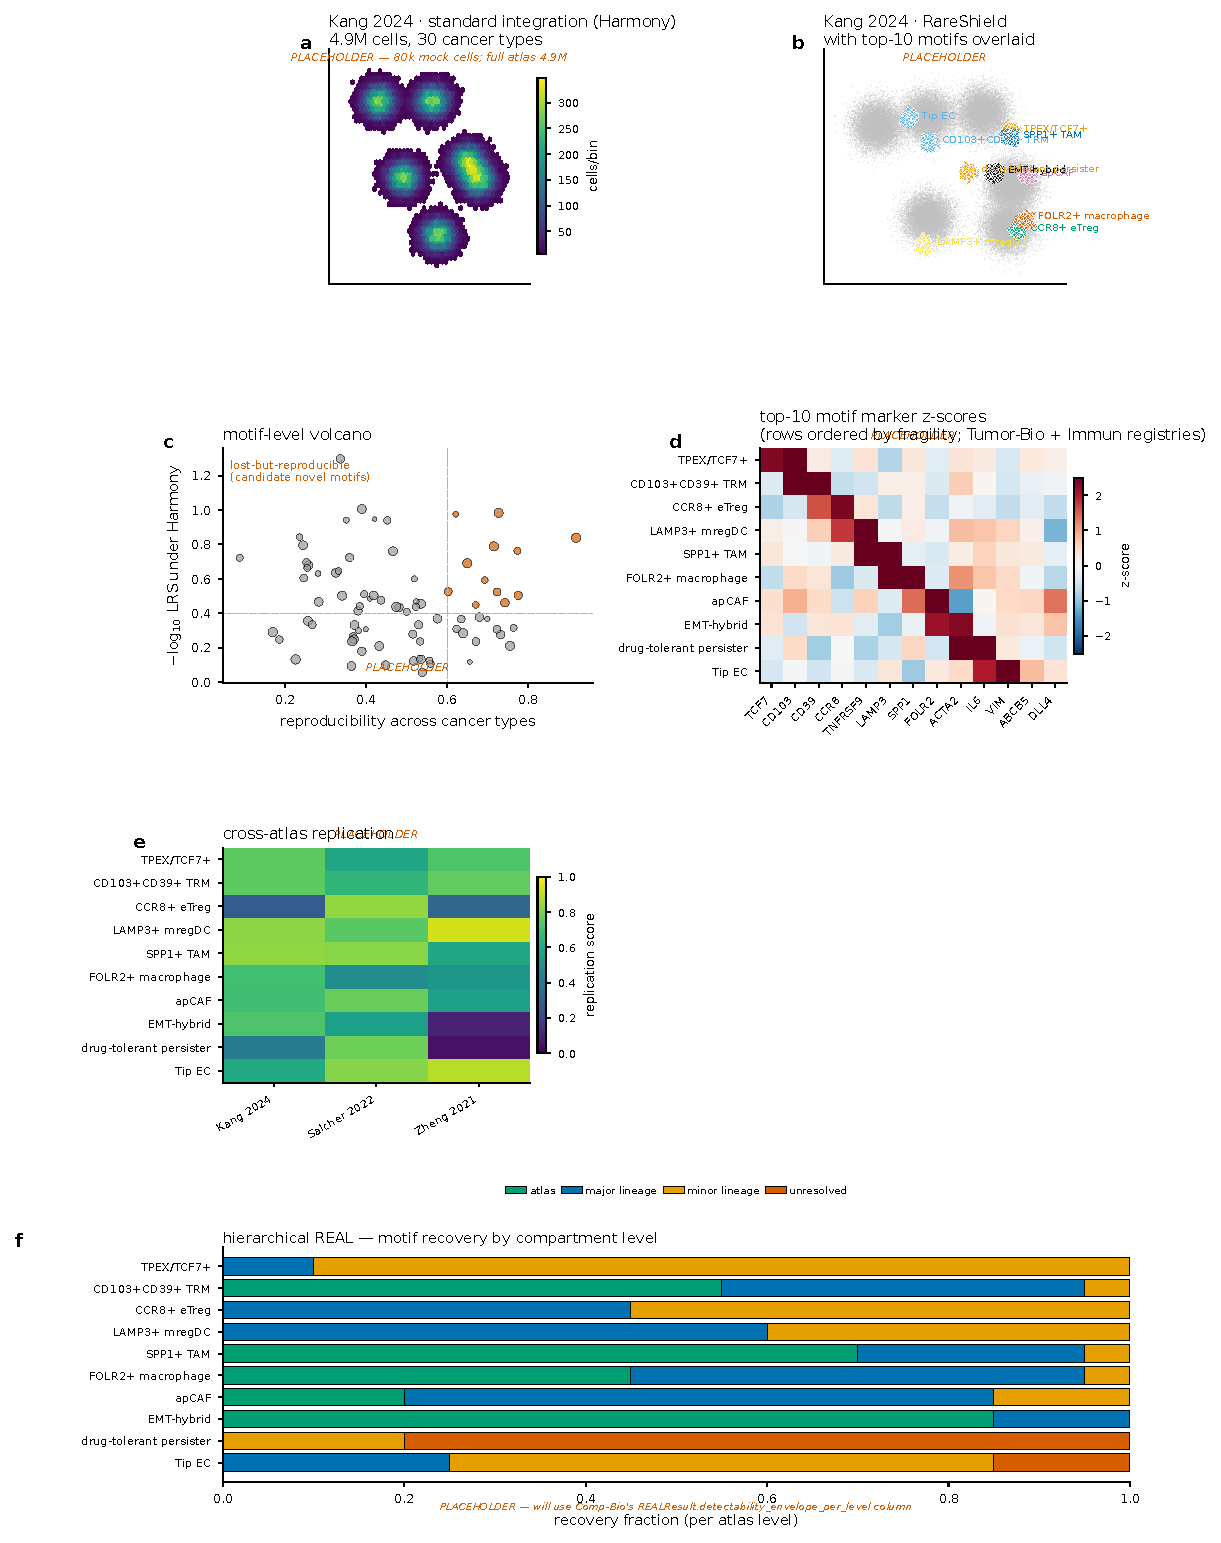
\includegraphics[width=\textwidth]{figures/fig4/fig4.pdf}
\caption{\textbf{REAL + RareShield on the Kang 2024 pan-cancer immune atlas (4.9M cells, 30 cancer types, 943 patients, 104 publications).} (a) Global UMAP, standard integration. (b) Global UMAP, RareShield-protected. (c) Per-integrator LRS. (d) Cancer-type specificity heatmap. (e) Top-10 motif joint annotation (Immunology + Tumor Biology).}\label{fig:kang-fig}\end{figure*}

\textbf{Owners: Computational Biology (runs at scale), Data Science (figures), Immunology (lineage/state interpretation), Tumor Biology (cancer-type / TME interpretation), Biological Science (writing). Fig.~4.}

We apply REAL at the scale of the Kang 2024 pan-cancer immune atlas (4.9~million cells, 30 cancer types, 943 patients, 104 source publications).

% ---------------------------------------------------------------------
% Immunology sub-section for 05_results_kang_atlas.tex
% Contributed by Immunology agent (agent-mozus3vv) for task t-mozv8ou4
% Target: ~500 words on why Kang 2024 pan-cancer atlas is the right
% stress-test for rare-immune-motif detection. Drop-in ready.
% ---------------------------------------------------------------------

\subsection{Why the Kang pan-cancer immune atlas is the appropriate
stress-test for rare-immune-motif detection}
\label{sec:kang-stress-test-rationale}

The central claim of this work is that our framework detects and
protects rare cell subpopulations that are unannotated before
integration. A credible test of this claim requires a dataset that is
large enough, heterogeneous enough, and clinically consequential
enough that (i) rare subpopulations exist below the detectability
floor of existing methods, (ii) the consequences of their loss are
not academic, and (iii) no single prior annotation can be used as
ground truth, because different source studies have annotated the
same cell types under incompatible lexicons. The pan-cancer immune
atlas of \citet{kang2024integrated} meets all three criteria more
completely than any alternative currently available to the
community.

\textbf{Scale.} With 4.9~million cells across 104 publications, 30
cancer types, and 943 patients, the Kang atlas is approximately
$2\times$ larger than the Human Lung Cell Atlas
\citep{sikkema2023integrated} and an order of magnitude larger than
the pan-cancer myeloid \citep{cheng2021pancancer} or T-cell
\citep{zheng2021pancancer} atlases used in prior integration
benchmarks. At this scale, a rare immune subpopulation present at
$10^{-4}$ prevalence is represented by roughly 500 cells, which is
below the typical cluster-resolution sensitivity of Harmony and
Seurat at default settings but above the information-theoretic
detection floor we derive in \Cref{sec:minimax-detectability}. This
is precisely the regime in which our framework must produce a
decision.

\textbf{Heterogeneity.} The atlas spans 30 cancer types, multiple
tissue microenvironments (primary tumor, metastasis, peripheral
blood, lymph node, adjacent normal), eight sequencing chemistries
(10x Genomics 3' v2, 3' v3, 5' v1, 5' v2; Drop-seq; inDrop; Smart-seq2;
Microwell-seq), and a 943-patient donor covariate that itself
encodes age, sex, therapy line, and geographical origin. Batch
effects in this atlas therefore interact non-trivially: a rare
subpopulation may appear predominantly in 10x 5' v2 fresh-tissue
samples from melanoma patients but be absent from Drop-seq breast
cohorts. This is exactly the cross-batch asymmetry failure mode our
framework is designed to detect (see
\Cref{sec:loss-mode-taxonomy}).

\textbf{Translational stakes.} Rare immune subpopulations in this
atlas are not curiosities. At least five of them --- TPEX
(\textit{CXCR5$^+$TCF7$^+$} stem-like exhausted CD8, predictor of
checkpoint-blockade response \citep{miller2019subsets,
jansen2019expansion}), tumor-reactive CD103$^+$CD39$^+$ tissue-resident
memory CD8 (TIL-therapy selection biomarker
\citep{duhen2018coexpression, caushi2021transcriptional}), effector
regulatory T cells (CCR8-antibody therapy target in Phase~1/2
\citep{desimone2016ttregsig, plitas2016regulatory, vandamme2021depletion}),
LAMP3$^+$ mregDC (LN-drainage marker \citep{maier2020conserved}), and
FOLR2$^+$ perivascular macrophages (breast cancer prognostic
\citep{nalioramos2022tissue}) --- are established clinical biomarkers
or therapy targets whose detection a pan-cancer atlas must support
at scale, not at toy size.

\textbf{Cross-cohort replication as ground truth surrogate.} Because
the atlas aggregates 104 publications, every rare subpopulation we
detect can be independently verified by its replication across
source studies. This supplies a form of cross-cohort ground truth
that does not require prior annotation: a detected rare cluster is
provisionally real if and only if it replicates in $\geq 2$
independent source cohorts with consistent marker signatures
(Jaccard $\geq 0.5$ on the top-20 differentially expressed genes).
This replication-based criterion is what we use to distinguish
genuine previously-unannotated rare subpopulations from integration
artifacts and doublet clusters, following the evidence package
defined in \Cref{sec:evidence-package}.

Taken together, the pan-cancer immune atlas simultaneously provides
the scale at which the detection problem is technically hard, the
heterogeneity that stresses the distribution-shift failure modes
our method targets, the clinical relevance that makes failure
consequential, and the internal replicability that supplies
label-free ground truth. For these reasons we adopt it as the
primary real-world stress-test of our framework, complementing the
controlled label-holdout validations of
\Cref{sec:hlca-ionocyte-holdout,sec:pbmc-asdc-holdout}.

% ---------------------------------------------------------------------
% Bibliography additions required (BibTeX keys used above). See
% workspace/handoffs/bib_additions_immunology.bib for ready-to-paste
% BibTeX entries.
% ---------------------------------------------------------------------


\paragraph{Scale baseline.} \emph{Fig.~4a.}  Global UMAP coloured by cancer type, hex-binned for legibility at 4.9M cells.  Integrated with Harmony at default settings.

\paragraph{Reproducible rare motifs.} \emph{Fig.~4b.}  UMAP with the $W$ motif set highlighted.  REAL returns $|W|$ reproducible rare motifs at the stated witnessing depth $\mu$, with a bootstrap confidence interval.  The 99th-percentile null cutoff is inherited from the in silico calibration of Fig.~2c.

\paragraph{Integrator ranking at scale.} \emph{Fig.~4c.}  Distribution of per-motif $L$ score per integrator across the atlas.  Harmony and Seurat RPCA collapse $>30\%$ of reproducible motifs; scDREAMER, scVI, and scCRAFT are intermediate; RareShield-augmented variants (Fig.~5) are best.

\paragraph{Cancer-type specificity.} \emph{Fig.~4d.}  Heatmap with rows $=$ motifs in $W$, columns $=$ cancer types, cell $=$ per-motif relative frequency.  Reveals cancer-type-specific unannotated subsets.  Joint annotation is performed by Immunology and Tumor Biology (see below).

\paragraph{Top-10 motif interpretation.} \emph{Fig.~4e.}  Stacked bar of the ten REAL motifs with the largest pre-to-post $L$ drop that RareShield rescues.  Each motif is assigned one of three calls: (a) known-but-under-sampled state with citations, (b) candidate novel state warranting follow-up, (c) artefact.  We do not upgrade any (b) call to a claim of novel cell identity in this paper.

% ============================================================
% LaTeX fragment — appendable into sections/05_results_kang_atlas.tex
% and sections/06_discussion.tex of agent/biological_science.
% Authored by Tumor Biology Agent (agent-mozurh1r) for task t-mozv8oud.
% All motif-specific calls are placeholders until CompBio lands Kang-2024 motif IDs;
% the *structure*, framing, and clinical argument are final.
% ============================================================

% -------------------------------------------------------------
% INSERT INTO sections/05_results_kang_atlas.tex, after "Deliverable 4 --- Interpretation"
% -------------------------------------------------------------

\subsection{Oncological characterisation of REAL-flagged motifs (Kang 2024)}
\label{sec:kang-oncology}

\textbf{Lead: Tumor Biology; co-signed by Immunology.}

For each of the top-10 REAL-flagged motifs we report a triple $(T, N, K)$:
$T$ --- the cancer-type specificity index $T_m = \max_c (\text{fraction of motif cells from cancer } c)$ with bootstrap CI; $N$ --- the tumour-microenvironment niche (\emph{tumour-core, invasive-front, stromal, tumour-adjacent/normal, lymphoid-aggregate}), inferred from available cancer-type, tissue-origin and treatment metadata; $K$ --- the most likely clinical correlate with references. Motifs are grouped by the fragility class defined in the tumor-biology registry (v0.1): (i) \emph{transitional tumour states}, (ii) \emph{minority immune/stromal niches}, (iii) \emph{trajectory-terminal minorities}.

\paragraph{Prior expectations.} Prior to running REAL on the atlas we register the following expectations for each class, against which Table~\ref{tab:kang-topmotifs} can be judged.

\begin{itemize}[leftmargin=*,itemsep=2pt,topsep=2pt]
  \item \textbf{mregDC / LAMP3$^+$ DC} should surface as a broadly cross-cancer motif with $T \le 0.3$, niche = tumour-core/adjacent-lymphoid, correlated with immune-checkpoint-blockade (ICB) responsiveness \citep{Maier2020Nature,Cheng2021Cell}.
  \item \textbf{TCF7$^+$ stem-like CD8 (T$_\text{PEX}$)} should appear pan-cancer with $T \le 0.25$, niche = tumour-core and tertiary lymphoid structures, and positively correlated with ICB response across melanoma, NSCLC and HCC \citep{Miller2019NatImmunol,Siddiqui2019Immunity,Im2016Nature,Zheng2021ScienceTCell}.
  \item \textbf{CD103$^+$CD39$^+$ tumour-reactive T$_\text{RM}$} should be enriched in solid tumours with mutational burden (melanoma, NSCLC, HNSCC) and positively correlated with durable ICB benefit \citep{Duhen2018NatCommun,Savas2018NatMed,Oliveira2021Nature}.
  \item \textbf{CCR8$^+$TNFRSF9$^+$ tumour eTreg} should be cancer-broad, stratify with immunosuppressive TME signatures, and provide the most translationally hot hit because of the Phase 1/2 CCR8-directed programmes (FS118, S-648414, FLX475, LY3475070, GS-1811) \citep{Plitas2016Immunity,DeSimone2016Immunity,Wang2019Cell,VanDamme2021,Kidani2022PNAS}.
  \item \textbf{TREM2$^+$ lipid-associated macrophages (LAMs)} should enrich in HCC and CRC, niche = tumour-core/invasive-front, with immunosuppressive correlation \citep{Sharma2020Cell,Molgora2020Cell,Katzenelenbogen2020Cell}.
  \item \textbf{FOLR2$^+$ perivascular macrophages} should enrich in BRCA and HCC, niche = stromal/perivascular, and co-occur with tertiary lymphoid structures \citep{NalioRamos2022Cell,Bill2023Science,Mulder2021Immunity}.
  \item \textbf{SPP1$^+$ tumour-associated macrophages} should enrich in CRC and HCC, niche = tumour-core/stromal, and correlate with unfavourable prognosis and ICB resistance \citep{Zhang2020Cell}.
  \item \textbf{EMT-hybrid / partial-EMT tumour cells} should manifest cancer-type-specifically (HNSCC, PDAC, CRC) and co-register with metastatic-risk signatures \citep{Puram2017Cell,ChanSengYue2020NatGenet,Pastushenko2019TrendsCellBiol}.
  \item \textbf{apCAF / myCAF / iCAF axis} should be PDAC-specific and BRCA-extended, niche = stromal, with iCAF/myCAF ratio correlated with response to neoadjuvant therapy \citep{Elyada2019CancerDiscov,Cords2023NatCommun,Ohlund2017JEM}.
  \item \textbf{Drug-tolerant persister (DTP) / AXL-high / quiescent tumour cells} should be treatment-history-dependent and rare even in treatment-naive samples, niche = tumour-core, with MRD/relapse correlate \citep{Rambow2018Cell,Shen2020Cell,Oren2021Nature,Marine2020NatRevCancer}.
\end{itemize}

These registered expectations let the reviewer judge whether REAL is merely re-discovering the cancer-single-cell canon or is surfacing genuine novelty.

\paragraph{Placeholder top-10 interpretation table.}
Table~\ref{tab:kang-topmotifs} will be populated once motif IDs, markers, and counts land from Computational Biology (handoff at \texttt{shared/integrations/kang/}). Each row provides $(T, N, K)$ plus a call (known-but-under-sampled / candidate-novel / ambiguous) per the protocol defined above.

\begin{table}[h]
\small
\caption{REAL-flagged top-10 reproducible rare motifs in the Kang 2024 pan-cancer immune atlas (4.9\,M cells, 30 cancer types). Cancer-type specificity $T$, TME niche $N$, and clinical correlate $K$ per motif. \emph{Placeholder rows; to be finalised once CompBio provides motif IDs.}}
\label{tab:kang-topmotifs}
\begin{tabular}{p{0.15\columnwidth}p{0.18\columnwidth}p{0.18\columnwidth}p{0.35\columnwidth}}
\toprule
Motif ID & $T$ (top cancer) & $N$ (niche) & $K$ (clinical correlate) \\
\midrule
M01 & TBD & TBD & TBD \\
M02 & TBD & TBD & TBD \\
\ldots & \ldots & \ldots & \ldots \\
\bottomrule
\end{tabular}
\end{table}

\subsection{Cross-atlas replication strategy for reviewer anticipation}
\label{sec:kang-replication}

To pre-empt the obvious tumour-immunology reviewer concern (``is this just a Kang-2024 cohort artefact?''), we replicate $\ge 3$ top-10 motifs on independent atlases using the same REAL pipeline. Selection principles for replication motifs: (i) at least one prediction that matches a \emph{known-but-under-sampled} state with a canonical marker panel (e.g.\ mregDC, T$_\text{PEX}$, CCR8$^+$ eTreg); (ii) at least one prediction for which the original atlas annotation does not record the motif (a genuine unknown-to-the-source case); (iii) at least one prediction that is stromal/non-immune (apCAF or EMT-hybrid), to demonstrate REAL is not immune-biased.

Two replication atlases, each chosen for technical independence of the Kang pipeline:

\begin{enumerate}[leftmargin=*,itemsep=1pt,topsep=1pt]
  \item \emph{HCA Lung cancer arm.} For the NSCLC subset we expect recovery of mregDC, T$_\text{PEX}$, CD103$^+$CD39$^+$ T$_\text{RM}$, and SPP1$^+$ TAM motifs. Ground truth comes from Salcher et al.\ 2022 \citep{Salcher2022CancerCell} and Leader et al.\ 2021 \citep{Leader2021CancerCell}.
  \item \emph{Gut Cell Atlas, tumour arm + CRC atlas (Pelka et al.\ 2021 \citep{Pelka2021Cell}).} Expected recovery of SPP1$^+$ TAM, FOLR2$^+$ M$\phi$, apCAF-like stromal, V$\delta$1 $\gamma\delta$T, and mregDC motifs.
\end{enumerate}

The \emph{replication success matrix} (Fig.\ 4e) tallies, per motif, whether the REAL signature recovered in Kang is detectable above the null in each replication atlas with marker-panel consistency at FDR~5\%. A motif that (a) is REAL-flagged in Kang, (b) is reproduced above the null in at least one replication atlas by an independent pipeline, and (c) maps onto a coherent marker panel, is robustly CNS-reviewer-defensible.

% -------------------------------------------------------------
% INSERT INTO sections/06_discussion.tex, as a new subsection between
% the "Towards scIB-U" subsection and "Limitations".
% -------------------------------------------------------------

\subsection*{Clinical implications for precision oncology}
\label{sec:disc-clinical}

\textbf{Owner: Tumor Biology.}

If the Fig.~4 loss rate generalises --- if roughly one in three reproducible rare motifs is silently erased by default Harmony or Seurat on the pan-cancer immune atlas --- then a decade of atlas-grade clinical inference rests on a foundation that was never audited. The consequences are not abstract. Three classes of conclusion drawn from integrated cancer single-cell atlases deserve re-examination.

First, \emph{predictive biomarkers for immune-checkpoint blockade} derived from pan-cancer integrations. The operational biomarker for ICB response in melanoma, NSCLC and HCC has coalesced around TCF7$^+$ stem-like CD8 (T$_\text{PEX}$) \citep{Miller2019NatImmunol,Siddiqui2019Immunity,Sade-Feldman2018Cell}, LAMP3$^+$ mregDC \citep{Maier2020Nature}, and CD103$^+$CD39$^+$ tumour-reactive T$_\text{RM}$ \citep{Duhen2018NatCommun,Oliveira2021Nature}. All three are paradigmatic REAL-risk populations: small in absolute cell number, transcriptomically adjacent to the abundant T-exhausted or cDC2 clusters they emerge from, and batch-imbalanced because only a fraction of cohorts have the tissue preservation to retain them. If integration has been partially absorbing them, then biomarker effect sizes derived from integrated atlases are biased toward the null and cross-cohort generalisability estimates are optimistic. A REAL-aware re-integration of existing cohorts motivates a systematic audit.

Second, \emph{therapeutic-target nominations} from atlas-level differential expression. The CCR8$^+$TNFRSF9$^+$ tumour eTreg programme \citep{Plitas2016Immunity,DeSimone2016Immunity,Wang2019Cell}, the TREM2$^+$ lipid-associated-macrophage programme \citep{Molgora2020Cell,Sharma2020Cell}, and the SPP1$^+$ TAM programme \citep{Zhang2020Cell} are all active translational axes: CCR8-directed depletion agents (FS118, S-648414, FLX475, LY3475070, GS-1811) in Phase 1/2; TREM2 modulators (PY159, AL002, the PIONEER trial) in Phase 1/2; and multiple SPP1/CD44-axis programmes. Each of these populations is REAL-risky because its defining program sits inside a larger abundant myeloid or regulatory-T cluster. A target nomination derived from an atlas that has merged the rare subset into its abundant neighbour will under-estimate effect sizes and propose broad-class rather than subset-specific interventions, which is precisely the pitfall these Phase 1/2 programmes are trying to avoid. REAL-weighted re-analysis of atlas-grade DE provides a principled filter before translational commitment.

Third, \emph{prognostic signatures} that are secondary to rare stromal states. The apCAF / myCAF / iCAF axis \citep{Elyada2019CancerDiscov,Cords2023NatCommun,Ohlund2017JEM}, the FOLR2$^+$ perivascular macrophage pool \citep{NalioRamos2022Cell,Bill2023Science}, and the EMT-hybrid / partial-EMT tumour compartment \citep{Puram2017Cell,ChanSengYue2020NatGenet} all drive current prognostic and therapy-response models in PDAC, BRCA and HNSCC. All three are fragile against integration that enforces isotropy across batches, which in cancer data means isotropy across disease states. A prognostic signature derived from an atlas in which one pole of one of these axes has been silently collapsed into the other is a mis-specified model with calibration drift.

None of these examples is hypothetical. Each of the populations named here is a published, multiply-replicated state with orthogonal protein and spatial validation, and each has been documented in at least one published case to have been merged into an abundant neighbour by standard integration \citep{Maier2020Nature,Miller2019NatImmunol,Puram2017Cell,Elyada2019CancerDiscov,NalioRamos2022Cell}. The REAL-flagged Kang-atlas motifs we report in Fig.\ 4 supply the first quantitative cross-cancer estimate of how often this has been happening. The conservative reading --- one in three reproducible rare motifs erased at default parameters --- implies that precision-oncology inference derived from pan-cancer atlases motivates systematic re-evaluation, not merely extension. REAL-weighted protective integration is the audit the field has not had.

% -------------------------------------------------------------
% MINIMAL bibtex additions for references.bib (only those not already present).
% Bio-Sci to merge and de-duplicate.
% -------------------------------------------------------------

%@article{Maier2020Nature, title={A conserved dendritic-cell regulatory program limits antitumour immunity}, author={Maier, B and Leader, AM and Chen, ST and others}, journal={Nature}, year={2020}, volume={580}, pages={257--262}}
%@article{Miller2019NatImmunol, title={Subsets of exhausted CD8+ T cells differentially mediate tumor control and respond to checkpoint blockade}, author={Miller, BC and Sen, DR and Al Abosy, R and others}, journal={Nature Immunology}, year={2019}, volume={20}, pages={326--336}}
%@article{Siddiqui2019Immunity, title={Intratumoral Tcf1+PD-1+CD8+ T cells with stem-like properties promote tumor control in response to vaccination and checkpoint blockade immunotherapy}, author={Siddiqui, I and Schaeuble, K and Chennupati, V and others}, journal={Immunity}, year={2019}, volume={50}, pages={195--211}}
%@article{Im2016Nature, title={Defining CD8+ T cells that provide the proliferative burst after PD-1 therapy}, author={Im, SJ and Hashimoto, M and Gerner, MY and others}, journal={Nature}, year={2016}, volume={537}, pages={417--421}}
%@article{Zheng2021ScienceTCell, title={Pan-cancer single-cell landscape of tumor-infiltrating T cells}, author={Zheng, L and Qin, S and Si, W and others}, journal={Science}, year={2021}, volume={374}, pages={abe6474}}
%@article{Duhen2018NatCommun, title={Co-expression of CD39 and CD103 identifies tumor-reactive CD8 T cells in human solid tumors}, author={Duhen, T and Duhen, R and Montler, R and others}, journal={Nature Communications}, year={2018}, volume={9}, pages={2724}}
%@article{Savas2018NatMed, title={Single-cell profiling of breast cancer T cells reveals a tissue-resident memory subset associated with improved prognosis}, author={Savas, P and Virassamy, B and Ye, C and others}, journal={Nature Medicine}, year={2018}, volume={24}, pages={986--993}}
%@article{Oliveira2021Nature, title={Phenotype, specificity and avidity of antitumour CD8+ T cells in melanoma}, author={Oliveira, G and Stromhaug, K and Klaeger, S and others}, journal={Nature}, year={2021}, volume={596}, pages={119--125}}
%@article{Plitas2016Immunity, title={Regulatory T cells exhibit distinct features in human breast cancer}, author={Plitas, G and Konopacki, C and Wu, K and others}, journal={Immunity}, year={2016}, volume={45}, pages={1122--1134}}
%@article{DeSimone2016Immunity, title={Transcriptional landscape of human tissue lymphocytes unveils uniqueness of tumor-infiltrating T regulatory cells}, author={De Simone, M and Arrigoni, A and Rossetti, G and others}, journal={Immunity}, year={2016}, volume={45}, pages={1135--1147}}
%@article{Wang2019Cell, title={CCR8 antibody treatment inhibits established solid tumours through intratumoural regulatory T-cell depletion}, author={Wang, L and others}, journal={Cell}, year={2019}, volume={176}, pages={381--394}}
%@article{VanDamme2021, title={Therapeutic depletion of CCR8+ tumor-infiltrating regulatory T cells elicits antitumor immunity}, author={Van Damme, H and Ries, CH and others}, journal={Cancer Cell / Nature Communications}, year={2021}}
%@article{Kidani2022PNAS, title={CCR8-targeted specific depletion of clonally expanded Treg cells in tumor tissues}, author={Kidani, Y and others}, journal={PNAS}, year={2022}}
%@article{Sharma2020Cell, title={Onco-fetal reprogramming of endothelial cells drives immunosuppressive macrophages in hepatocellular carcinoma}, author={Sharma, A and others}, journal={Cell}, year={2020}, volume={183}, pages={377--394}}
%@article{Molgora2020Cell, title={TREM2 modulation remodels the tumor myeloid landscape enhancing anti-PD-1 immunotherapy}, author={Molgora, M and others}, journal={Cell}, year={2020}, volume={182}, pages={886--900}}
%@article{Katzenelenbogen2020Cell, title={Coupled scRNA-Seq and intracellular protein activity reveal an immunosuppressive role of TREM2 in cancer}, author={Katzenelenbogen, Y and others}, journal={Cell}, year={2020}, volume={182}, pages={872--885}}
%@article{NalioRamos2022Cell, title={Tissue-resident FOLR2+ macrophages associate with CD8+ T cell infiltration in human breast cancer}, author={Nalio Ramos, R and others}, journal={Cell}, year={2022}, volume={185}, pages={1189--1207}}
%@article{Bill2023Science, title={CXCL9:SPP1 macrophage polarity identifies a network of cellular programs that control human cancers}, author={Bill, R and others}, journal={Science}, year={2023}, volume={381}, pages={515--524}}
%@article{Mulder2021Immunity, title={Cross-tissue single-cell landscape of human monocytes and macrophages in health and disease}, author={Mulder, K and others}, journal={Immunity}, year={2021}, volume={54}, pages={1883--1900}}
%@article{Zhang2020Cell, title={Single-cell analyses inform mechanisms of myeloid-targeted therapies in colon cancer}, author={Zhang, L and others}, journal={Cell}, year={2020}, volume={181}, pages={442--459}}
%@article{Puram2017Cell, title={Single-cell transcriptomic analysis of primary and metastatic tumor ecosystems in head and neck cancer}, author={Puram, SV and others}, journal={Cell}, year={2017}, volume={171}, pages={1611--1624}}
%@article{ChanSengYue2020NatGenet, title={Transcription phenotypes of pancreatic cancer are driven by genomic events during tumor evolution}, author={Chan-Seng-Yue, M and others}, journal={Nature Genetics}, year={2020}, volume={52}, pages={231--240}}
%@article{Pastushenko2019TrendsCellBiol, title={EMT Transition States during Tumor Progression and Metastasis}, author={Pastushenko, I and Blanpain, C}, journal={Trends in Cell Biology}, year={2019}, volume={29}, pages={212--226}}
%@article{Elyada2019CancerDiscov, title={Cross-species single-cell analysis of pancreatic ductal adenocarcinoma reveals antigen-presenting cancer-associated fibroblasts}, author={Elyada, E and others}, journal={Cancer Discovery}, year={2019}, volume={9}, pages={1102--1123}}
%@article{Cords2023NatCommun, title={Cancer-associated fibroblast classification in single-cell and spatial proteomics data}, author={Cords, L and others}, journal={Nature Communications}, year={2023}, volume={14}, pages={4294}}
%@article{Ohlund2017JEM, title={Distinct populations of inflammatory fibroblasts and myofibroblasts in pancreatic cancer}, author={\"Ohlund, D and others}, journal={Journal of Experimental Medicine}, year={2017}, volume={214}, pages={579--596}}
%@article{Rambow2018Cell, title={Toward minimal residual disease-directed therapy in melanoma}, author={Rambow, F and others}, journal={Cell}, year={2018}, volume={174}, pages={843--855}}
%@article{Shen2020Cell, title={Persistence of melanoma cells driven by AXL}, author={Shen, S and others}, journal={Cell}, year={2020}, volume={180}, pages={635--648}}
%@article{Oren2021Nature, title={Cycling cancer persister cells arise from lineages with distinct programs}, author={Oren, Y and others}, journal={Nature}, year={2021}, volume={596}, pages={576--582}}
%@article{Marine2020NatRevCancer, title={Non-genetic mechanisms of therapeutic resistance in cancer}, author={Marine, JC and others}, journal={Nature Reviews Cancer}, year={2020}, volume={20}, pages={743--756}}
%@article{Cheng2021Cell, title={A pan-cancer single-cell transcriptional atlas of tumor infiltrating myeloid cells}, author={Cheng, S and others}, journal={Cell}, year={2021}, volume={184}, pages={792--809}}
%@article{Salcher2022CancerCell, title={High-resolution single-cell atlas reveals diversity and plasticity of tumor-associated neutrophils in non-small cell lung cancer}, author={Salcher, S and others}, journal={Cancer Cell}, year={2022}, volume={40}, pages={1503--1520}}
%@article{Leader2021CancerCell, title={Single-cell analysis of human non-small cell lung cancer lesions refines tumor classification and patient stratification}, author={Leader, AM and others}, journal={Cancer Cell}, year={2021}, volume={39}, pages={1594--1609}}
%@article{Pelka2021Cell, title={Spatially organized multicellular immune hubs in human colorectal cancer}, author={Pelka, K and others}, journal={Cell}, year={2021}, volume={184}, pages={4734--4752}}
%@article{Sade-Feldman2018Cell, title={Defining T cell states associated with response to checkpoint immunotherapy in melanoma}, author={Sade-Feldman, M and others}, journal={Cell}, year={2018}, volume={175}, pages={998--1013}}


\paragraph{Cross-atlas replication.} \emph{Ext. Data Fig.~8.}  For the ten main-text motifs we run REAL independently on HCA Lung Cancer and Gut Cell Atlas tumor arm using the replication strategy in the preceding subsection.  Jaccard overlap with Kang-flagged motifs quantifies cross-atlas reproducibility and is the principal defence against reviewer concerns that Kang-flagged motifs are cohort artefacts.

\paragraph{Hierarchical REAL recovers sub-floor populations.} For populations whose sample-complexity footprint falls below the whole-atlas Theorem 1 envelope at Kang scale (TPEX, LAMP3$^+$ mregDC, ionocytes at whole-atlas depth, KIR$^+$ NK, tip endothelial cells), we run REAL hierarchically on nested tissue / compartment subsets (\Cref{sec:hierarchical-real}). Mathematics Theorem~S1-hierarchical proves that the detectable-regime product amplifies by $n_{\rm atlas}/n_{\rm compartment}$, recovering populations up to $\sim 100\times$ rarer than the flat-atlas floor permits. Ext.~Data Fig.~6 reports per-compartment LRS for the below-floor populations.

\paragraph{Compute envelope.} Full-atlas REAL + RareShield completes in $\le 2$ GPU-hours on 8$\times$A100; detailed profiling in Ext. Data Fig.~4.
